% ==============================================================================
% 前言 (Preface)
% ==============================================================================

\chapter*{前言}
\addcontentsline{toc}{chapter}{前言}
\markboth{前言}{前言}
\label{sec:preface}
\renewcommand{\thefigure}{\arabic{figure}}\setcounter{figure}{0}
\renewcommand{\thetable}{\arabic{table}}\setcounter{table}{0}

许多职业都需要某种形式的编程。会计师为电子表格编写公式与宏；音乐家为合成器编程；作家为文字处理软件配置自动化脚本；网页设计师为样式表编写规则。当我们为本书第一版写下这些话时（1995--2000年），读者或许会觉得这种观点颇具前瞻性甚至带有未来主义色彩；而时至今日，编程早已成为一项不可或缺的基本技能，层出不穷的书籍、在线课程、中小学（K-12）课程都在竭力满足这一需求，其宗旨无一例外是提升人们的职场竞争力。

然而，典型的编程课程往往传授的是一种“瞎碰乱试，直到能跑为止”（tinker until it works）的试错方法。一旦代码碰巧产生预期的输出，学生们便欢呼雀跃：“它跑起来了！”然后草草收工。令人遗憾的是，这句话也是计算机领域流传最广、代价最为沉重的“最短谎言”——它耗费了无数人一生中数不清的宝贵光阴。与此截然相反，本书将全部重心聚焦于培养优良的编程习惯，无论是面向职业程序员还是专业开发者。

所谓“优良的程序设计”，我们指的是一种自始至终、贯穿每个阶段与步骤、依赖于系统性思考、周密规划与透彻理解的软件构建方法。为了强调这一点，我们称之为\term{系统性程序设计}（systematic program design）以及\term{经系统设计的程序}。至关重要的是，后者清晰地阐明了其所需功能背后的原理与合理性。此外，优秀的程序设计还能带来一种美学上的成就感；一个优秀程序的优雅程度，堪比历经岁月淘洗的经典诗篇，或是一张旧时代经典的黑白摄影杰作。简而言之，随意编码与优良程序设计的差异，正如餐垫纸上的蜡笔涂鸦与美术馆中传世油画之间的悬殊差距。

诚然，本书不可能把每个人都雕琢成绘画大师。但是，如果不是深信以下两点，我们绝不会花费整整十五年的心血来撰写这第二版：

\begin{quote}
\centering
\large\textbf{每个人都能学会设计程序} \\[1ex]
以及 \\[1ex]
\large\textbf{每个人都能体会到创造性设计所带来的成就感与乐趣。}
\end{quote}

事实上，我们的观点甚至更为深远：

\begin{quote}
\centering
\large\textbf{程序设计——而非单纯的编码——理应在通识博雅教育中享有与数学和语言技能同等重要的核心地位。}
\end{quote}

一位即使日后再也不写一行代码的学生，只要系统学习过程序设计，也必将掌握具有普遍适用性的通用问题求解技能，亲身经历一种高度创造性的智力活动，并学会鉴赏一种全新的美学形式。本前言的后续部分将深入阐述我们所说的“系统性设计”的真谛、何人能以何种方式从中获益，以及我们如何展开全方位的教学。


% ------------------------------------------------------------------------------
\section*{系统性程序设计}
\addcontentsline{toc}{section}{系统性程序设计}
\label{sec:preface:systematic_design}
% ------------------------------------------------------------------------------

程序需要与人（被称为用户）以及其他程序（此时我们称之为服务器与客户端组件）进行交互。因此，任何功能相对完备的程序都由诸多构件组成：一些负责处理输入，一些负责生成输出，还有一些负责在两者之间架起桥梁。我们选择将\term{函数}（functions）作为最基本的构建单元，这是因为每个人在初等代数阶段都接触过函数，而且最简单的程序本质上就是这样的函数。设计的关键在于：发现需要哪些函数、如何将它们连接起来，以及如何利用基本元素构建出这些函数。

在此背景下，“系统性程序设计”融合了两个核心概念：\term{设计配方}（design recipes）与\term{逐步求精}（iterative refinement）。设计配方是本书作者的独创，正是它使得逐步求精在编程初学阶段成为可能。

\begin{notebox}[思想渊源]
本书的设计理念深受 Michael Jackson 创立的 COBOL 程序构建方法启发，并得益于与 Daniel Friedman 关于递归的深入交流、与 Robert Harper 关于类型论的切磋，以及与 Daniel Jackson 关于软件设计的广泛探讨。
\end{notebox}

设计配方既适用于构建完整的程序，也适用于设计单独的函数。本书只涉及两种针对完整程序的设计配方：一种针对图形用户界面（GUI）程序，另一种针对批处理程序。相比之下，针对函数的设计配方则丰富多样：针对原子形式的数据（如数字）；针对不同类别数据的枚举；针对以固定方式复合其他数据的数据；针对有限但任意大小的数据，等等。

函数级别的各个设计配方都遵循一个统一的设计流程。图~\ref{fig:design_recipe_steps} 展示了其六个核心步骤。每个步骤的标题指明了预期的阶段性产物；其下的“指示”则指明了关键的思考与实践活动。在几乎每一个阶段，\textbf{示例}都扮演着核心角色。在步骤~1 选定数据表示时，写下具体的示例可以验证现实世界中的信息是如何被编码为数据的，以及数据又是如何被解释为现实信息的。步骤~3 要求解题者必须通过具体的场景实例，透彻理解目标函数在特定输入下应当计算出什么结果。这种理解在步骤~5（定义函数）时将得到充分利用。最后，步骤~6 要求将这些示例转化为自动化测试代码，以确保函数在已知案例上能够正确无误地工作。在现实数据上运行该函数，还可能进一步揭示预期与实际结果之间的其他偏差。

\begin{figure}[htbp]
  \centering
  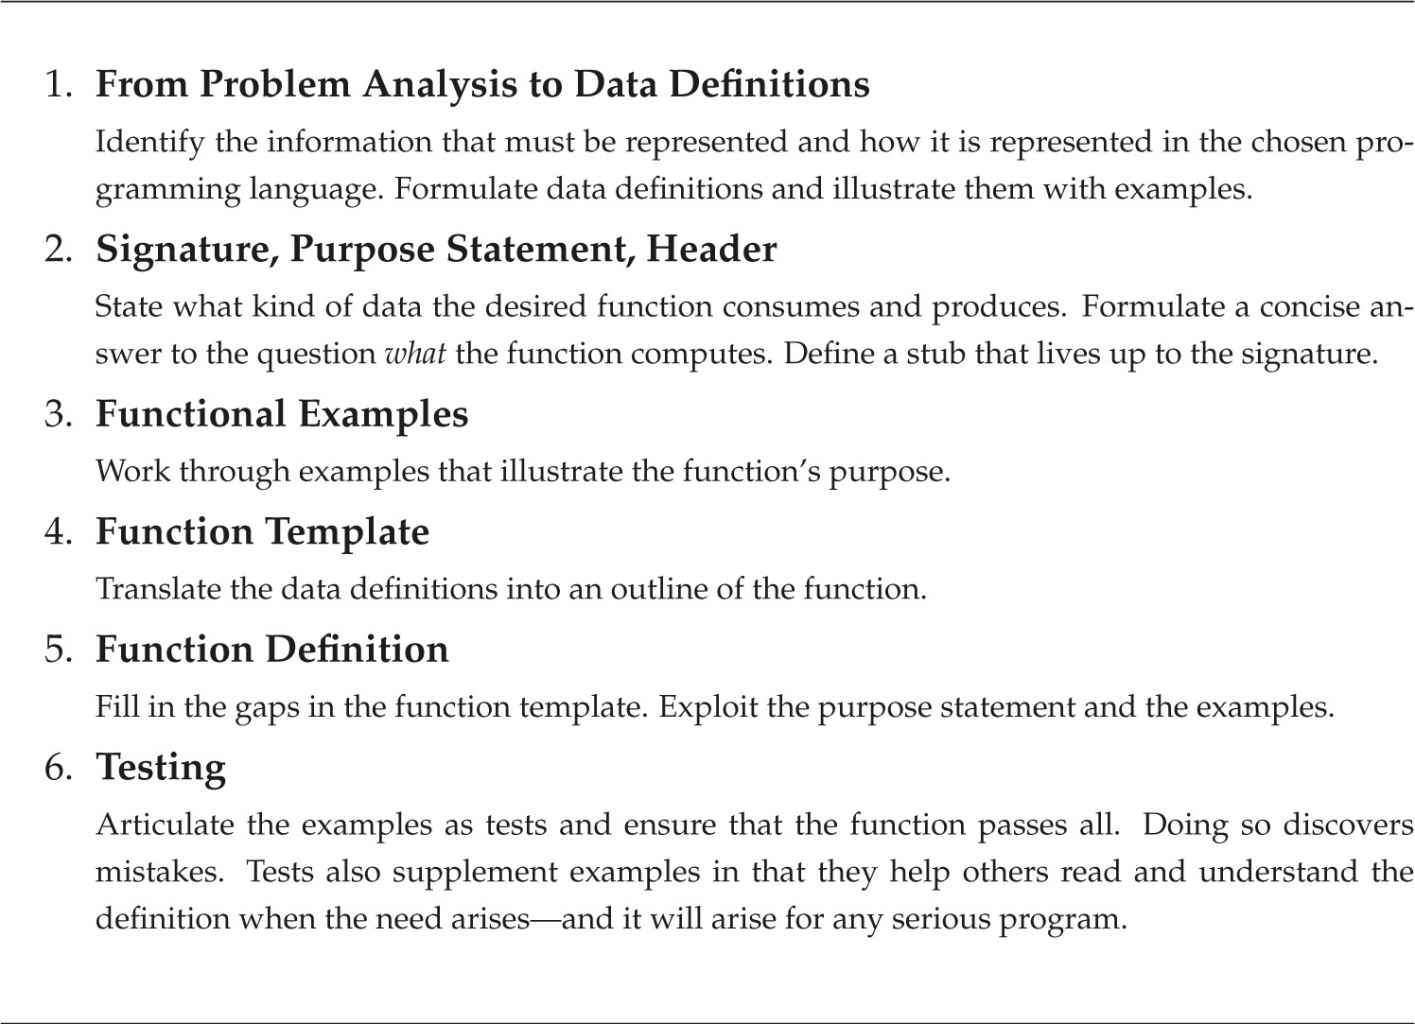
\includegraphics[width=0.88\textwidth]{images/00001.jpeg}
  \caption{函数设计配方的核心步骤}
  \label{fig:design_recipe_steps}
\end{figure}

\begin{notebox}[教师建议]
建议让学生将图~\ref{fig:design_recipe_steps} 的核心步骤抄写在索引卡片（卡片纸）的一面。当学生在解题中陷入困境不知所措时，让他们拿出卡片，并指出他们当前停滞在哪个步骤上。
\end{notebox}

设计流程的每一步都配有针对性极强的关键提问。对于某些步骤——例如构造功能示例或提炼函数模板——这些提问会直接依托于数据定义。回答这些问题几乎能够自然而然地生成中间产物。这种“脚手架”（scaffolding）机制在进入整个流程中唯一的创造性步骤——完成函数定义的编写时，将展现出巨大的威力。即便利在此时，在绝大多数情况下依然有规律可循、有法可依。

\begin{notebox}[教师建议]
在整个设计流程中，最为关键的问题集中在步骤~4 与步骤~5。建议让学生用他们自己的语言，将这两个步骤的核心问题抄写在索引卡片的背面。
\end{notebox}

这种方法的创新之处在于：它为初学者阶段的程序创建了明确的\term{中间产物}。当一个新手卡壳时，专家或导师可以通过审查现有的中间产物来诊断问题所在。导师通过抛出设计流程中的通用提问，引导新手进行自我审视并自主修正错误。这种\textbf{自我赋能}（self-empowering）的思维训练过程，正是单纯的随意编码与真正的程序设计之间的分水岭。

\term{逐步求精}（Iterative Refinement）旨在应对现实问题的复杂性与多面性。试图一蹴而就、一次性把所有细节都做对，几乎是不可能的。计算机科学家从物理科学中借鉴了逐步求精的思想来攻克这一设计难题。其本质思想是：首先剥离掉所有非本质的细枝末节，先为保留下来的核心问题找到一个清晰的解决方案。随后，在每一次求精步骤中，重新引入一个之前忽略的细节，并尽可能复用现有的解决方案来解决扩展后的新问题。重复（即迭代）这一求精过程，最终便能得到一个完备的解决方案。

从这个意义上说，程序员就像是一位“微型科学家”。科学家针对现实世界的某种理想化模型进行建模，以便对其做出预测。只要模型的预测与观测吻合，一切便顺利成章；一旦预测与实际观测出现偏差，科学家就会修正并提炼模型以缩小差距。同理，当程序员接到一项任务时，他们会完成初步设计，将其转化为代码，交由真实用户进行评估，随后通过持续的逐步求精，直至程序的行为与目标产品高度吻合。

本书通过两种不同的方式引入逐步求精。由于当程序结构变复杂时通过求精进行设计尤为关键，本书在第四部分随着问题难度的大幅提升，正式系统地引入了该技术。此外，在本书前三部分中，我们也通过在后续章节中针对同一问题提出越来越复杂的变体，潜移默化地运用逐步求精——即在一个章节中解决问题的核心，在后续章节中引入新概念的同时，为该问题增添相匹配的细节维度。


% ------------------------------------------------------------------------------
\section*{DrRacket 与教学语言}
\addcontentsline{toc}{section}{DrRacket 与教学语言}
\label{sec:preface:drracket_languages}
% ------------------------------------------------------------------------------

学习设计程序需要反复的亲身动手实践。正如不弹琴绝不可能成为钢琴家一样，不编写实际程序并让它们正确运行，任何人都不可能成为优秀的程序设计者。因此，本书配备了一套极简而精悍的软件支持环境：一门用于书写程序的编程语言，以及一个让读者能够像编辑文本一样编写程序并直接运行的集成开发环境。

许多我们在生活中遇到的人都说他们渴望学会写代码，接着便询问应该学习哪门编程语言。鉴于媒体对某些流行语言的大肆宣传，提出这样的问题并不令人意外，但这种问法从根本上就走入了误区。在当下时髦的某种流行语言中学习编程，往往是在为学生未来的挫败埋下伏笔。技术世界的流行风潮极其短暂。一本典型的“X 天精通某语言”的书籍或速成班，根本无法传授能够迁移到下一波潮流语言中的核心计算原理。更糟糕的是，工业级语言本身的繁杂语法与特殊机制，往往严重干扰了可迁移技能的吸收——无论是在表达解决方案的思维层面，还是在处理程序错误与调试的认知层面。

\begin{notebox}[教师建议]
对于非零基础受众或高阶课程，在教学中亦可直接使用工业界现成语言配合本设计配方进行讲授。
\end{notebox}

与此相反，学习设计程序的核心在于研习根本原理与获得可终身迁移的技能。理想的教学编程语言必须全心全意服务于这两个目标，然而市面上现存的任何工业语言都无法胜任。其致命瓶颈在于：初学者在尚未全面掌握语言语法之前就会犯错，而工业级语言的报错诊断机制却总是假定程序员已经通晓整门庞大的语言体系。结果就是，晦涩难懂的报错信息常常令初学者如坠云雾，大受打击。

我们的解决方案是：从我们专门量身定制的教学语言开始起步，这门语言被称为\term{初学学生语言}（Beginning Student Language，简称 \term{BSL}）。这门语言本质上就是学生在初等代数课程中所习得的“算术与代数符号系统”。它涵盖了函数定义、函数调用以及条件表达式的记法，并且支持表达式的任意嵌套。由于这门语言的规模极小，其报错诊断信息即使基于整门语言的规则给出，对于仅具备初等代数知识的读者而言依然一目了然、清晰易懂。

\begin{notebox}[教师建议]
教师可以向学生解释：BSL 本质上就是初等代数，只是在此基础上扩充了若干额外的数据类型（如字符串、布尔值、图像等），以及定义在这些数据之上的一系列内置函数。
\end{notebox}

一旦学生完全掌握了基于结构的程序设计原则，便可以进阶到\term{中级学生语言}（Intermediate Student Language，简称 \term{ISL}）以及更高阶的教学方言，统称为 \term{*SL}。本书利用这些进阶方言来传授抽象设计原则与通用递归算法。我们坚信，通过这一系列循序渐进的教学语言的淬炼，能够为读者未来在广泛的专业编程语言（如 JavaScript、Python、Ruby、Java 等）中构建高质量软件提供无可比拟的深厚底蕴。

\begin{notebox}[关于 Racket 的说明]
这套教学语言系列全部基于 Racket 实现——Racket 是我们专门为了“打造编程语言”而开发的一门现代编程语言。如今，Racket 已经走出象牙塔，在工业界的各类实际场景中大显身手，从游戏开发到射电望远镜阵列的运行控制皆有其身影。尽管教学语言从 Racket 中汲取了诸多语法与设计元素，但本书并不专门教授 Racket。当然，彻底学完本书的学生，完全可以轻而易举地过渡并熟练使用 Racket。
\end{notebox}

在编程环境的选择上，我们面临着与编程语言同样的困境。面向专业工程师的现代开发环境，其复杂程度堪比巨型客机的驾驶舱，密密麻麻的仪表盘与控件足以让任何初次启动该软件的新人感到窒息。初学程序员真正需要的，是一架双座单发螺旋桨式教练机，让他们能够全神贯注地操练基本飞行技能。为此，我们量身打造了 \term{DrRacket}——一个专为初学者设计的交互式集成开发环境。

DrRacket 凭借两个极其简洁的交互窗格，全力支持富有趣味性、反馈即时的探索式学习：位于上半部分的\term{定义区}（definitions area）用于编写函数与常量定义；位于下半部分的\term{交互区}（interactions area）则允许程序员即时求值并测试引用了这些定义的表达式。在这样的环境中，探索“如果……会怎样”（what-if）的假设场景就像在电子表格软件中那样轻松自如。从初次接触的第一分钟起，读者就可以从经典的计算器式操作开始实验，并迅速过渡到对图像、文本及各种丰富数据形态的动态计算。

像 DrRacket 这样的交互式开发环境在两个关键维度上极大地降低了学习门槛。首先，它让初学者能够直接操控真实数据。由于省去了从文件或外设中读取输入信息的繁杂代码，初学者不必将宝贵精力虚耗在理解底层 I/O 机制上。其次，这种布局在架构上严格地将“数据及其内部计算逻辑”与来自现实世界的“输入/输出展现”分离开来。在当今软件工程界，这种解耦思想被视为系统化软件设计的基石，并被赋予了闻名遐迩的名字：\term{模型-视图-控制器}（Model-View-Controller，简称 \term{MVC}）架构。通过在 DrRacket 中学习，初学者从起步的第一天起，便在潜移默化中自然吸收了这一现代软件工程的核心范式。


% ------------------------------------------------------------------------------
\section*{可以迁移的技能}
\addcontentsline{toc}{section}{可以迁移的技能}
\label{sec:preface:skills_transfer}
% ------------------------------------------------------------------------------

通过学习系统性程序设计所习得的技能，具有双向迁移的深远价值。首先，它们自然适用于广义上的所有通用编程任务，乃至针对电子表格、音乐合成器、网页样式表甚至是文字处理器的自动化开发。我们的长期教学观察表明，图~\ref{fig:design_recipe_steps} 所示的设计流程能够无缝迁移到几乎任何现代编程语言中，并且无论是编写 10 行的小函数，还是驾驭 10,000 行的大型软件模块，它都同样行之有效。要在跨越不同编程语言与不同规模问题时熟练运用该设计流程，确实需要一番反思与内化；然而一旦该流程化为你的第二天性，其所带来的巨大生产力与质量收益将在各个方面显现。

此外，学习设计程序还意味着掌握两种具有普适价值的核心素养。程序设计无疑能够传授与数学（尤其是代数与几何）相同的严谨分析能力。然而与传统数学不同的是，与程序打交道是一种高度主动、富于互动性的学习方式。编写软件能够给予即时的正反馈，从而激发持续的探索、实验与自我评估。最终的产物通常是生动交互的软件作品，与传统教科书中枯燥单调的死记硬背练习相比，这能极大地增强学生的成就感与自信心。

除了强化数学思维之外，程序设计还是一门关于\textbf{分析性阅读与精确写作}的绝佳训练。哪怕是最小的程序设计任务，最初都是以文字应用题（word problem）的形式呈现的。缺乏扎实的阅读理解与分析能力，就绝不可能设计出能够解决复杂现实问题的优质程序。反之，程序设计方法强制要求创作者必须用规范、精确的语言来清晰阐述其思考过程。事实上，如果学生真正领会了设计配方的精髓，他们在思维表达与条理性方面的提升将远超其他任何技能。

为了说明这一点，不妨重温图~\ref{fig:design_recipe_steps} 中总结的设计流程。它要求设计者必须按部就班地：
\begin{enumerate}
  \item 分析问题陈述（通常以文字应用题的形式给出）；
  \item 抽象地提取并精确表达其核心概念与本质；
  \item 用具体的典型示例来验证并具象化这种本质；
  \item 基于前述分析制定清晰的设计大纲与规划；
  \item 依据预期的目标输出对设计产物进行客观评估；
  \item 根据未通过的测试用例与逻辑检查对产物进行系统修正。
\end{enumerate}

每一步都需要严谨的分析、精确的描述、高度的专注以及对细节的一丝不苟。任何一位经验丰富的企业家、工程师、记者、律师或科学家，都会深切认同上述技能在其日常核心工作中是何等不可或缺。在纸面上和 DrRacket 中亲身实践程序设计，正是习得这些宝贵素养的一条充满乐趣与智力美感的途径。

同样，逐步求精的设计方法绝不仅限于计算机科学与软件构建。建筑师、作曲家、作家以及各领域的专业人士亦是如此行事。他们的创作始于脑海中的灵感火花，并通过某种媒介勾勒其核心轮廓。随后他们在稿纸上反复斟酌推敲，直至最终作品尽可能完美地映射出其最初的心智构想。在将构思落于纸面的过程中，他们所运用的技巧与我们完全内化的设计配方如出一辙：或是通过素描绘画，或是通过文字修辞，或是通过指尖琴键，来展现建筑的风骨、刻画人物的性格或编织动人的旋律。使他们在迭代开发过程中保持高效产出的秘诀在于：他们已经将基本的设计配方化为本能，并能在面对具体情境时精准挑选出最适宜的工具。


% ------------------------------------------------------------------------------
\section*{本书的结构与组成}
\addcontentsline{toc}{section}{本书的结构与组成}
\label{sec:preface:structure}
% ------------------------------------------------------------------------------

本书的宗旨是引领没有任何编程经验的初学者步入系统化程序设计的殿堂。与此并行，本书提出了一种关于计算的\term{符号视角}（symbolic view of computation），这是一种专门阐明“程序作用于数据时的内部运作机制”的心智模型。粗略地说，这种方法推广并升华了学生在小学算术与初中代数中所学的运算规则。不过读者大可放心，DrRacket 内置了一个强大的机制——\term{代数单步求值器}（algebraic stepper），它能够一步一脚印地将这些计算推导过程以直观可视的方式完整展现出来。

全书主体由六个大部分组成，各部分之间穿插了五个“插曲”（intermezzo），并由“序幕”（Prologue）与“尾声”（Epilogue）首尾呼应。各大主要部分专注于传授核心程序设计思维，而各个插曲则介绍与编程机制和计算理论相关的补充概念与工具。

\begin{itemize}
  \item \textbf{序幕（Prologue）}是对纯粹编程的一次快速领略。它向读者展示了如何在教学语言中编写一个简单的火箭降落动画。完成之后，任何初学者在感到大开眼界、信心倍增的同时，也难免会感到些许手足无措。因此，序幕末尾的要点总结阐述了为什么脱离设计的随意编码是不可取的，以及循序渐进的系统化设计方法如何消除每个初学者必然经历的畏难心理。至此，全书核心舞台正式拉开序幕：
  
  \item \textbf{第一部分：固定大小的数据（Part I）}借助简单明了的案例讲解系统性设计的最核心概念。其核心立论是：程序设计者通常对程序需要消费与生成什么样的数据有初步的理解；因此，系统化的设计方法必须从对流入和流出程序的数据描述中提取尽可能多的指导线索。为了由浅入深，本部分从原子数据（数字、图像等）起步，循序渐进地引入描述数据的各种新形态：区间、枚举、分类数据、结构体以及它们的复合结构。
  
  \item \textbf{插曲 1（Intermezzo 1）}详尽剖析初学学生语言（BSL）的底层全貌：词汇表、文法规则及其运行语义。计算机科学家将这些称为语法（syntax）与语义（semantics）。程序设计者借助这一严谨的计算模型，能够准确预测其代码在运行时的求值行为，并高效分析诊断运行错误。
  
  \item \textbf{第二部分：任意大小的数据（Part II）}在第一部分的基础上展开延伸，引入了表达能力最强、最为实用的数据形态：任意大小的复合数据（列表）。第一部分中嵌套数据结构的深度和广度在代码中是固定的；本部分展示了一种精妙的通用化推广，带领我们跨越到任意大小的数据世界，随后重点转向处理此类数据的系统化程序设计。
  
  \item \textbf{插曲 2（Intermezzo 2）}引入了一种用于书写大规模复杂数据的紧凑而强大的表达记法：引用（quotation）与反引用（anti-quotation）。
  
  \item \textbf{第三部分：抽象（Part III）}敏锐地指出第二部分中编写的许多函数在结构上高度相似。优秀的编程语言绝不应强迫程序员一遍遍撰写大同小异的代码；相反，优良的语言必将提供消除此类冗余相似性的利器。计算机科学家将消除相似性的步骤及其产物统称为\term{抽象}（abstraction），并深知抽象能够成倍提升程序员的生产力。因此，本部分全面系统地传授创建与使用高阶抽象的设计配方。
  
  \item \textbf{插曲 3（Intermezzo 3）}承担着双重任务。一方面，它深入阐释了\term{词法作用域}（lexical scope）这一核心概念——即编程语言如何将每个名称严格绑定到程序员能够通过静态审查代码找到的唯一对应定义；另一方面，它介绍了一个包含丰富抽象机制的实用库，包括现代语言中常见的 \code{for} 循环推导式。
  
  \item \textbf{第四部分：交织数据（Part IV）}对第二部分的数据形态进行了更宏大的推广，并正式将“逐步求精”这一核心思维范式纳入设计方法工具箱中。
  
  \item \textbf{插曲 4（Intermezzo 4）}通过直观生动的实例，解释了为什么在所有现代计算机编程语言中十进制浮点数的运作机制常常出人意料。每一位抱负远大的未来程序员都必须掌握这些关于底层数字表示的关键事实。
  
  \item \textbf{第五部分：生成型递归（Part V）}增添了一项崭新的设计原则。虽然结构化设计与抽象足以应对绝大多数日常编程任务，但面对某些棘手问题时，它们偶尔会导致程序性能不足——即结构化设计的函数可能需要耗费过多时间或算力才能得出最终答案。因此，计算机科学家会设计出巧妙依托问题领域专属洞察的算法（如快速排序或二分搜索）。本部分展示了如何系统化地设计这一大类经典的生成型算法。
  
  \item \textbf{插曲 5（Intermezzo 5）}借助第五部分的经典案例，生动展示了计算机科学家是如何严谨分析与思考算法性能（时间与空间开销）的。
  
  \item \textbf{第六部分：累加器（Part VI）}为设计者的工具箱增添了终极秘诀：\term{累加器}（accumulators）。通俗地说，累加器为函数引入了“上下文记忆”。引入记忆机制能够大幅提升前四部分中结构化设计函数的执行效率；而对于第五部分中的复杂算法，累加器往往是能否在有限时间内求出答案的决定性分水岭。
  
  \item \textbf{尾声（Epilogue）}对全书体系进行了全景式的总结评估，并为有志于继续攀登计算高峰的读者指明了进阶方向。
\end{itemize}

自学读者应当通读全书，从第一页按部就班地学至最后一页。我们之所以强调“切实操练”，是因为读者应当动手解答全书所有的练习题，或者至少确保自己彻底清楚如何解答它们。

同样，任课教师应尽可能多地覆盖全书内容，从序幕一直贯彻至尾声。根据我们数十年的教学经验，这在完整学期中是完全切实可行的。通常，我们会在学期课程中布置一个大型且趣味盎然的综合项目（例如一个完整的交互式电子游戏）。然而我们也充分理解，在特定教学学时限制下可能需要做出针对性裁剪，且不同教师的教学风格对本书的取舍亦有所不同。

图~\ref{fig:book_dependencies} 为希望灵活选读本书内容的读者提供了一份清晰的导航图。该图展示了各个部分与插曲之间的逻辑依赖关系。实线箭头表示严格的强依赖关系（例如学习第二部分必须先掌握第一部分）；虚线箭头则主要作为建议参考（例如跳过序幕并不会影响后续主体章节的学习）。

\begin{figure}[htbp]
  \centering
  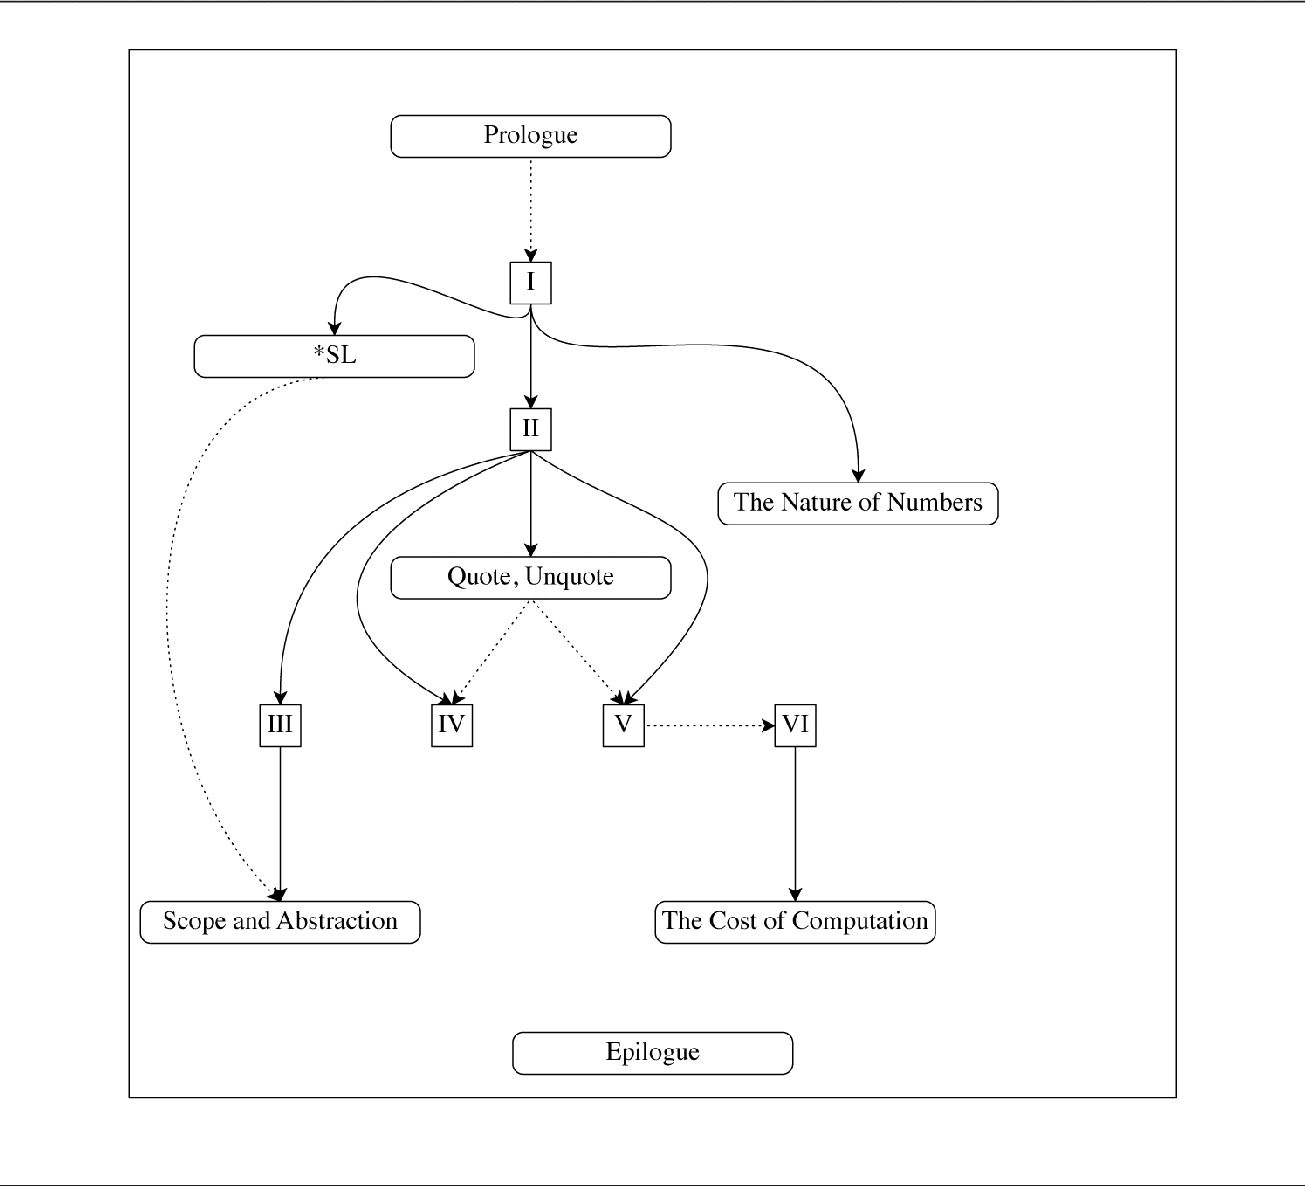
\includegraphics[width=0.88\textwidth]{images/00002.png}
  \caption{全书各部分与各插曲之间的依赖关系图}
  \label{fig:book_dependencies}
\end{figure}

基于该依赖图，我们为不同的教学场景推荐三种可行的学习路径：
\begin{itemize}
  \item \textbf{高中课程}：建议教师尽可能覆盖第一部分与第二部分，并在期末安排一个小型综合项目（如开发一款图形小游戏）。
  \item \textbf{大学学季制（Quarter）课程}：建议重点讲授第一部分、第二部分、第三部分与第五部分，并涵盖关于教学语言语义及词法作用域的插曲。
  \item \textbf{大学学期制（Semester）课程}：若希望尽早向学生揭示程序设计中的性能权衡，推荐在讲完第一和第二部分后，直接衔接第六部分中不依赖第五部分的累加器内容，随后讨论插曲~5，并在此视角下全面展开全书其他内容的教学。
\end{itemize}

\paragraph{螺旋式案例主题的持续迭代}
本书在全书各章节的例题与习题中反复回归若干经典主题。例如，“虚拟电子宠物”（virtual pets）贯穿了第一部分的始终，甚至在第二部分再度登场；又如，第一和第二部分分别从不同角度探讨了交互式文本编辑器的架构实现；图结构算法在第五部分登场后，立刻在第六部分中被再次深入剖析。这种反复回归同一主题的用意，在于从侧面潜移默化地引入并强化“逐步求精”的思想。我们强烈建议任课教师布置这些主题连续的系列习题，或结合自身教学特色设计类似的螺旋进阶习题序列。


% ------------------------------------------------------------------------------
\section*{两版之间的差异}
\addcontentsline{toc}{section}{两版之间的差异}
\label{sec:preface:differences}
% ------------------------------------------------------------------------------

《程序设计方法》第二版相较于第一版，在以下几个核心维度上做出了重大革新：

\begin{enumerate}
  \item \textbf{严格区分完整程序的设计与单个函数的设计}。具体而言，本版重点聚焦于两类典型程序架构：事件驱动程序（主要是图形用户界面 GUI 程序，也包括分布式网络程序）与批处理程序。
  
  \item \textbf{程序的构建明确划分为“自顶向下的规划阶段”与“自底向上的实现阶段”}。我们清晰地展示了外部库接口如何决定特定程序构件的代码形态。尤为突出的是，程序设计的最早阶段会直接产出一张\term{愿望清单}（wish list）。虽然愿望清单的概念在第一版中已初见端倪，但第二版将其确立为一项核心设计法则。
  
  \item \textbf{愿望清单中每个条目的落地实现，都严格遵循函数设计配方}，这构成了全书六大主体部分的核心内容。
  
  \item \textbf{结构化设计的一个决定性法则，是定义由若干子函数组合而成的复杂函数}。这种\term{组合式设计}（design-by-composition）在批处理程序的世界中尤为重要。与生成型递归相似，它需要灵光一闪的洞察力——即敏锐地意识到：由前一个函数生成中间数据结构、再由后一个函数对其进行处理，能够极大地简化整体设计。这种方法同样依赖愿望清单，但提出这些愿望需要针对中间数据定义进行富有远见的架构设计。第二版在书中精心穿插了大量针对组合式设计的专题训练。
  
  \begin{notebox}[致意]
  我们由衷感谢 Kathi Fisler 提醒我们重视组合式设计在现代教学中的关键地位。
  \end{notebox}
  
  \item \textbf{全面内置现代自动化测试支持}。虽然测试始终深植于我们的设计哲学之中，但教学语言与 DrRacket 直到 2002 年（第一版出版后不久）才从底层完备支持了自动化测试工具（如 \code{check-expect}）。新版彻底依托这套现代化的测试支持体系，使测试贯穿于教学的每一环节。
  
  \item \textbf{完全移除了命令式程序设计（imperative programming）的内容}。第一版的旧章节依然可以在线免费获取。这部分材料经过现代化重构后，将收录在本书的姊妹篇《How to Design Components》（如何设计组件）中。
  
  \item \textbf{全书案例与习题全面采用现代化的教学包（teachpacks）}。首选的引入方式是在代码中通过 \code{require} 显式导入，同时也完全兼容在 DrRacket 菜单中手动加载。
  
  \item \textbf{在若干专业术语与符号记号上进行了重要革新}：
  
  \begin{table}[htbp]
    \centering
    \small
    \begin{tabular}{ll}
      \hline
      \textbf{第二版（Second Edition）} & \textbf{第一版（First Edition）} \\
      \hline
      签名（\code{signature}） & 契约（\code{contract}） \\
      分类数据（\code{itemization}） & 联合（\code{union}） \\
      \code{'()} & \code{empty} \\
      \code{\#true} & \code{true} \\
      \code{\#false} & \code{false} \\
      \hline
    \end{tabular}
    \caption{第一版与第二版核心术语及记号对照表}
    \label{tab:edition_differences}
  \end{table}
  
  最后三项符号的更新，极大地优化了列表在引用（quotation）语法下的表达一致性与可读性。
\end{enumerate}


% ------------------------------------------------------------------------------
\section*{致谢}
\addcontentsline{toc}{section}{致谢}
\label{sec:preface:acknowledgments}
% ------------------------------------------------------------------------------

\subsection*{第一版致谢}

有四位先驱应当获得我们最崇高的谢意：Robert ``Corky'' Cartwright，他与第一作者共同开创了莱斯大学（Rice University）经典入门先导课程的雏形；Daniel P. Friedman，正是他在 1984 年力邀第一作者重写经典著作《The Little LISPer》（亦由 MIT Press 出版），从而点燃了整个项目的最初火种；John Clements，他亲手设计、实现并持续维护着 DrRacket 中不可或缺的代数单步求值器；以及 Paul Steckler，他始终忠实地为团队提供强有力的支持，为我们的编程工具链贡献良多。

本书的诞生还得益于众多亲朋好友与同行学者的鼎力相助，他们在各自的课堂中试用了早期讲义，并对草稿给出了详尽深入的宝贵意见。我们由衷感激他们的热情支持与耐心包容：Ian Barland、John Clements、Bruce Duba、Mike Ernst、Kathi Fisler、Daniel P. Friedman、John Greiner、G{\'e}raldine Morin、John Stone 以及 Valdemar Tamez。

莱斯大学 Comp 210 课程的数十届学子在教学中试用了本书的早期书稿，并从各个维度为本书的完善做出了贡献。此外，参加过我们 TeachScheme! 师资培训工作坊的众多骨干教师在自己的中小学课堂上积极践行了早期讲义，并慷慨反馈了大量的宝贵建议。作为这些热忱贡献者的杰出代表，我们特别鸣谢：Barbara Adler 女士、Stephen Bloch 博士、Karen Buras 女士、Jack Clay 先生、Richard Clemens 博士、Kyle Gillette 先生、Marvin Hernandez 先生、Michael Hunt 先生、Karen North 女士、Jamie Raymond 先生与 Robert Reid 先生。Christopher Felleisen 耐心地同他的父亲一起通读了本书前几个部分，为我们提供了来自年轻初学者的最直接洞见。Hrvoje Blazevic（当时在 ``LPG/C Harriette'' 轮船上担任船长）、犹他大学的 Joe Zachary 以及印第安纳大学的 Daniel P. Friedman 在本书第一版第一次印刷中指出了若干勘误，我们在此次修订中已全部修正。谨向所有人致以最诚挚的谢忱。

最后，Matthias 谨向 Helga 致以最深切的感激，感谢她多年来的无限包容，为一个总是在神游天外的丈夫与父亲营造了温暖的港湾。Robby 由衷感谢黄幸惠（Hsing-Huei Huang）的全心支持与由衷鼓励；没有她的陪伴，他将一事无成。Matthew 感谢袁雯（Wen Yuan）始终如一的温暖守候与悠扬持久的音乐陪伴。Shriram 深深感激 Kathi Fisler 的坚定支持、包容耐心与诙谐妙语，以及她全程深度参与到这一宏大项目中所付出的心血。

\subsection*{第二版致谢}

正如在 2001 年那样，我们怀着由衷的敬意感谢 John Clements 设计、验证、实现并维护了 DrRacket 的代数单步求值器。这项长跑他已经坚持了近二十年，单步求值器早已成为全书概念讲解与教学互动中无可替代的支柱级工具。

在过去数年间，多位学术界同仁研读了书稿的各个版本并提出了宝贵的改进意见。我们由衷感激与以下诸位学者富有启发性的思想交流与探讨：Kathi Fisler（伍斯特理工学院与布朗大学）、Gregor Kiczales（不列颠哥伦比亚大学）、Prabhakar Ragde（滑铁卢大学）以及 Norman Ramsey（塔夫茨大学）。

多年来，数以千计的教师参加了我们的各类师资培训工作坊，并反馈了海量的教学心得。其中，Dan Anderson、Stephen Bloch、Jack Clay、Nadeem Abdul Hamid 与 Viera Proulx 的贡献尤为卓著，在此我们特别向他们在第二版编写过程中所发挥的重要作用致以最诚挚的敬意。

Guillaume Marceau 在与 Kathi Fisler 及 Shriram 的紧密合作下，耗费数月心血对 DrRacket 的错误诊断提示机制进行了脱胎换骨式的深入研究与重构。我们对其卓越的工作致以崇高敬意。

Celeste Hollenbeck 堪称我们所遇过的最不可思议的审校读者。在彻底读懂行文之前，她从不知疲倦地反复推敲质疑；在一节内容尚未能完全支撑其核心论点、结构尚未严丝合缝、段落句子尚未浑然一体之前，她绝不轻言放行。对她所付出的超凡努力，我们谨致以最深厚的由衷谢意。

我们还要向以下诸位致谢，感谢他们对第二版各阶段草稿提出的中肯批评与建设性意见：Saad Bashir、Steven Belknap、Stephen Bloch、Joseph Bogart Tomas Cabrera、Estevo Castro、Stephen Chang、Jack Clay、Richard Cleis、John Clements、Mark Engelberg、Christopher Felleisen、Sebastian Felleisen、Vladimir Gaji{\'c}、Adrian German、Ryan Golbeck、Jane Griscti、Alberto E. F. Guerrero、Nadeem Abdul Hamid、Wayne Iba、Jordan Johnson、Marc Kaufmann、Gregor Kiczales、Eugene Kohlbecker、Jackson Lawler、Ben Lerner、Elena Machkasova、Jay Martin、Jay McCarthy、Ann E. Moskol、Paul Ojanen、Klaus Ostermann、Alanna Pasco、S. Pehlivanoglu、David Porter、Norman Ramsey、Ilnar Salimzianov、Brian Schack、Tubo Shi、Stephen Siegel、Kartik Singhal、Marc Smith、Dave Smylie、Vincent St-Amour、{\'E}ric Tanter、Sam Tobin-Hochstadt、Manuel del Valle、David Van Horn、Mitch Wand、Roelof Wobben 与 Andrew Zipperer。

htdp.org 网站上优雅清晰的在线排版布局出自 Matthew Butterick 之手，他专门为我们的在线文档量身设计了这套排版样式。

最后，我们由衷感谢麻省理工学院出版社（MIT Press）的资深编辑 Ada Brunstein 与 Marie Lufkin Lee，她们慷慨许可我们在互联网上公开打磨这第二版《How to Design Programs》。我们亦诚挚感谢 MIT 的 Christine Bridget Savage 与 Westchester Publishing Services 的 John Hoey 统筹全书最后的出版印制流程；John Donohue、Jennifer Robertson 以及 Mark Woodworth 在文稿文字编辑方面完成了令人赞叹的杰出工作。
